% Draw a comparator in the rows given by #1 and #2, with a horizontal
% displacement of #3
\def\comp#1#2#3{%
  \draw (#1)+(#3,0) node {$\bullet$};
  \draw (#2)+(#3,0) node (n2) {$\bullet$};
  \draw[thick] (#1)+(#3,0) -- (n2.center);
}

%%%%%%%%%%

\section{Example: Quick Sort}

In this section we build a circuit of small threads.  The circuit inputs a
steam of |Int|s (with the end of stream signalled by the channel closing), and
then outputs a sorted version of that stream (and closes the channel to
indicate that).  The circuit is not the most practical way to sort numbers;
but it illustrates various ideas.

More precisely, we will write a  definition with the following signature
%
\begin{scala}
  def qSort(in: ??[Int], out: !![Int]): ThreadGroup = ...
\end{scala}
%
The function will produce a |ThreadGroup| that, when run, performs the
sorting.  The sorting will be based on the Quicksort algorithm.  That
algorithm is recursive, so the |qSort| function will also be recursive.

%%%%%

\framebox{Names for threads -- explain notation}

Suppose the input stream is empty.  Then |qSort| should just close its output
port to signal an empty output stream.  This can be achieved using the
following outline.
%
\begin{scala}
  def qSort(in: ??[Int], out: !![Int]): ThreadGroup = thread("QSort"){
    attempt{
      val pivot = in?()
      ...
    }{
      out.endOfStream // We've received no data, so just close
    }
  }
\end{scala}
%
The command |attempt{p}{q}| acts like~|p|, but if that throws a |Stopped|
exception, it executes~|q|.  Thus if the initial attempt to input on |in|
fails, the function performs |out.endOfStream|.

We now consider the resursive case.  Suppose the first input succeeds, giving
a value stored in |pivot|.  We then create two recursive |qSort| threads, that
will deal with values less than |pivot|, and at least pivot, respectively.  In
addition, a controller thread ties things together.  The controller
%
\begin{itemize}
\item Continues to input on |in|, passing values to the appropriate recursive
  |qSort| thread;

\item When |in| is closed, closes the channels to the recursive |qSort|s to
  signal the end of their input streams;

\item Receives the outputs from the recursive |qSorts|, and passes them along
  on |out|, along with |pivot|, in the appropriate order.
\end{itemize}
%
The following diagram illustrates how the controller communicates with the
recursive |qSort| processes.
%
\begin{center}
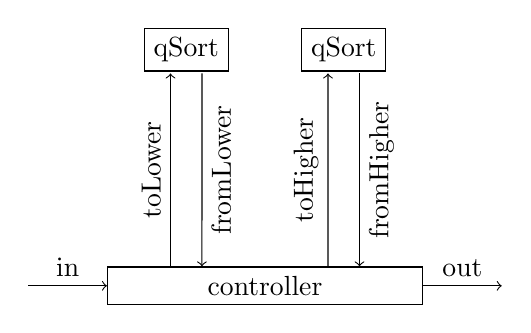
\begin{tikzpicture}
\draw (0,0) node[draw, minimum width=40mm] (controller) {\scalashape controller};
\draw[->] (controller.west) ++ (-1,0) -- 
   node[above]{\scalashape in} (controller.west);
\draw[<-] (controller.east)++(1,0)  -- 
   node[above]{\scalashape out} (controller.east);
%
\draw (controller) ++ (-1,3) node[draw] (rec1) {\scalashape qSort};
\draw (rec1.south)++(-0.2,0.1) node (rec1In) {};
\draw[->] (controller.north) ++ (-1.2,0.0) -- 
  node[above,sloped] {\scalashape toLower} (rec1In);
\draw (rec1.south)++(0.2,0.1) node (rec1Out) {};
\draw[<-] (controller.north) ++ (-0.801,0) -- 
  node[below,sloped] {\scalashape fromLower} (rec1Out);
%
\draw (controller) ++ (1,3) node[draw] (rec2) {\scalashape qSort};
\draw (rec2.south)++(-0.2,0.1) node (rec2In) {};
\draw[->] (controller.north) ++ (0.8,0.0) -- 
  node[above,sloped] {\scalashape toHigher} (rec2In);
\draw (rec2.south)++(0.2,0.1) node (rec2Out) {};
\draw[<-] (controller.north) ++ (1.2,0) -- 
  node[below,sloped] {\scalashape fromHigher} (rec2Out);
\end{tikzpicture}
\end{center}

%%%%%

The following definition implements this strategy.
%
\begin{scala}
  def qSort(in: ??[Int], out: !![Int]): ThreadGroup = thread("QSort"){
    attempt{
      val pivot = in?()
      val toHigher, toLower, fromHigher, fromLower = new SyncChan[Int]
      // Main controller thread.
      def controller = thread("Controller"){
        repeat{ val n = in?(); if(n < pivot) toLower!n else toHigher!n }
	toHigher.endOfStream; toLower.endOfStream
        repeat{ out!(fromLower?()) }; out!pivot; repeat{ out!(fromHigher?()) }
        out.endOfStream
      }      
      // Put the system together and run it.
      run(controller || qSort(toHigher, fromHigher) || qSort(toLower, fromLower))
    }{ out.endOfStream } // We've received no data, so just close
  }
\end{scala}

%%%%%  

Testing is an important part of programming.  Since concurrent programs tend
to be harder than sequential ones, testing is particularly important.

A general strategy for testing is to generate some random data, run the
parallel program on it, run a sequential program on it, and check that the two
give the same answer.  This can be repeated many times.  Of course, this
assumes that we have a correct sequential program for the same problem.  (In
fact, this strategy is also useful for testing sequential programs, where we
have a, typically simple, implementation that we are sure is correct, but we
want to test a more sophisticated program against it.)

%% Here's a strategy for testing:
%% %
%% \begin{enumerate}
%% \item Pass in values from an array~|xs| of random numbers;
%% \item Receive the outputs into an array~|ys|;
%% \item Check that |ys| is indeed a sorted version of~|xs|;
%% \item Repeat many times.
%% \end{enumerate}

The following code achieves this.
%
\begin{scala}
  import scala.util.Random
  val MaxSize = 100; val Max = 100
  def doTest{
    val size = Random.nextInt(MaxSize)
    val xs = Array.fill(size)(Random.nextInt(Max))
    val ys = new Array[Int](size)
    val in, out = new SyncChan[Int]
    def sender = thread("sender"){ for(x <- xs) in!x; in.endOfStream }
    def receiver = thread("receiver"){ var i = 0; repeat{ ys(i) = out?(); i += 1 } }
    run(sender || qSort(in, out) || receiver)
    assert(xs.sorted.sameElements(ys))
  }
\end{scala}
%
The |doTest| function performs a single test.  If uses an array |xs| of
size~|size|, where |size| is picked randomly in the range
$\interval{0}{\sm{MaxSize}}$; each element of |xs| is picked randomly in the
range $\interval{0}{\sm{Max}}$.  The |sender| thread sends the elements
of~|xs| to the |qSort| network on the |in| channel, then signals the end of
the stream.  The |receiver| thread receives the outputs from |qSort|, and
stores them in~|ys|.  The final line tests whether a sorted version of |xs|
(sorted using the |sorted| function from the Scala |Array| class) contains the
same elements as the outputs.

We can then run |doTest| many times:
%
\begin{scala}
  for(i <- 0 until 1000){ doTest; if(i%10 == 0) print(".") }
\end{scala}
%
This also intermittently prints a dot on the screen; this means that if the
system deadlocks for some reason, we will spot that it has got stuck!

%%%%%%%%%%%%%%%%%%%%%%%%%%%%%%%%%%%%%%%%%%%%%%%%%%%%%%%%%%%%

\heading{Practical 1: sorting networks}

The first practical asks you to implement various sorting algorithms using
fine-grained concurrency.  

Each sorting network will be built from \emph{comparators}: simple
two-element sorting components.  A comparator can be pictured as below: 
%
\begin{center}
\begin{tikzpicture}[scale = 0.8, >=angle 90,shorten >=1pt]
\node at (0,0.6) {comparator};
\draw (-2,-0.5) rectangle (2,1.5);
\node (x1) at (-5, -0.2) {$x_1$};
\node (x0) at (-5, 1.2) {$x_0$};
\draw[->] (x1) -- node[above]{ $in_1$} (-2,-0.2);
\draw[->] (x0) -- node[above]{ $in_0$} (-2,1.2);
\node (y1) at (6.5,-0.2) {$y_1 = max(x_0,x_1)$};
\node (y0) at (6.5,1.2) {$y_0 = min(x_0,x_1)$};
\draw[->] (2,-0.2) -- node[above]{ $out_1$} (y1);
\draw[->] (2,01.2) -- node[above]{ $out_0$} (y0);
\end{tikzpicture}
\end{center}
%
The comparator has two input channels, $in_0$ and $in_1$, and two output
channels, $out_0$ and $out_1$.  If it inputs $x_0$ and~$x_1$, it outputs their
minimum on~$out_0$ and their maximum on~$out_1$.

%%%%%

Below is a sorting network for four inputs using five comparators.
%
\begin{center}
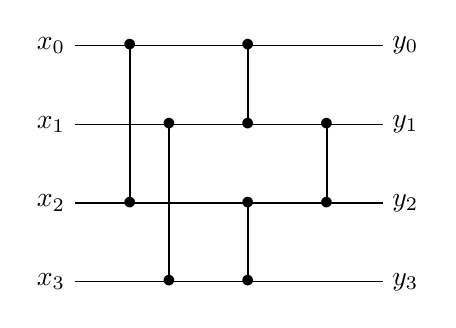
\begin{tikzpicture}
\draw (0,0) node (x0) {$x_0$};
\draw (0,-1) node (x1) {$x_1$};
\draw (0,-2) node (x2) {$x_2$};
\draw (0,-3) node (x3) {$x_3$};
\draw (4.5,0) node (y0) {$y_0$};
\draw (4.5,-1) node (y1) {$y_1$};
\draw (4.5,-2) node (y2) {$y_2$};
\draw (4.5,-3) node (y3) {$y_3$};
\draw (x0) -- (y0);
\draw (x1) -- (y1);
\draw (x2) -- (y2);
\draw (x3) -- (y3);
\comp{x0}{x2}{1}  \comp{x1}{x3}{1.5}
\comp{x0}{x1}{2.5}  \comp{x2}{x3}{2.5}
\comp{x1}{x2}{3.5}
\end{tikzpicture}
\end{center}
%
The first four comparators direct the smallest and largest values to the top
and bottom outputs; the final comparator sorts out the middle two values.

%%%%%%%%%%%%%%%%%%%%%%%%%%%%%%%%%%%%%%%%%%%%%%%%%%%%%%%%%%%%

\heading{Ordering of actions}

It is sometimes useful to consider an ordering over actions (memory reads and
writes, and sends and receives of messages) that talks about the order in
which those actions must happen.

We will write $a \preceq a'$, and say $a$ \emph{happens before}~$a'$, if (in a
particular execution of the program), $a'$ occur after, or simultaneously
with, $a$.

Note that if $a$ and $a'$ are a send and the corresponding receive over a
synchronous channel, then $a \preceq a'$ and $a' \preceq a$, so the relation
is not antisymmetric. 

%%%%%


We write $\equiv$ for the equivalence relation induced by~$\prec$:
\[
a \equiv a' \iff a \preceq a' \land a' \preceq a.
\]
This means that $a$ and~$a'$ happen at the same time, e.g.~the send and
receive on a synchronous channel.

We write $\prec$ for the strict version of~$\preceq$:
\[
a \prec a' \iff a \preceq a' \land a \not\equiv a.
\]
This means that $a$ happens strictly before~$a'$.

Formally, $\preceq$ is a preorder, i.e.~a transitive, reflexive order such
that:
%
\begin{itemize}
\item
If $a$ and $a'$ are actions of a single thread, and $a$ precedes $a'$, then $a
\prec a'$ (so $a \preceq a'$ but $a' \not\preceq a$);

\item
If $a$ is a send and $a'$ is the corresponding receive, then $a \preceq a'$
(regardless of whether the communication is over a synchronous or asynchronous
channel);  

\item
If $a$ is a receive and $a'$ is the corresponding send, and the communication
is over a synchronous channel, then $a \equiv a'$.
\end{itemize}

Note that some pairs of actions may be unrelated by~$\preceq$, so they can
happen in either order (necessarily in different threads).  In such cases, we
need to be sure that either order is acceptable --- i.e.~there is no race
condition. 

%%%%%%%%%%%%%%%%%%%%%%%%%%%%%%%%%%%%%%%%%%%%%%%%%%%%%%%%%%%%

\heading{Data-less channels}

It is sometimes useful to use a channel communication solely for
synchronisation between threads, rather than to pass any data.

This can be achieved in SCL using a channel that passes data of type
\SCALA{Unit}, the trivial type that contains a single value~\SCALA{()}.  

For example:
\begin{scala}
val c = new SyncChan[Unit]
run(thread{ print("Hello "); c!() } || thread{ c?(); println("world") })
\end{scala}

% This usage corresponds to simple events in CSP. 
We can reason using the happens-before relation.
\[
\sm{print("Hello")} \prec \sm{c!()} \equiv \sm{c?()} \prec \sm{println("world")}.
\]

The use of |!| and |?| could be reversed (but not with a buffered channel).

%%%%%%%%%%%%%%%%%%%%%%%%%%%%%%%%%%%%%%%%%%%%%%%%%%%%%%%%%%%%

\heading{Caching and compiler optimisations}

Recall that multiprocessor machines may cache variables, and that Java does
not guarantee that the caches will be kept coherent, so two concurrent
threads may operate independently on their own cached copies of the same
variable!  And further, the compiler is allowed to optimise the code to
something semantically equivalent as a sequential program.  The Java Memory
Model
%% \footnote{%
  %% \url{http://www.cs.umd.edu/~pugh/java/memoryModel/jsr-133-faq.html}.}
defines this more formally.

However, when two threads synchronise on a channel communication, any writes
made by one thread before the synchronisation are guaranteed to be visible to
the other thread after the synchronisation.  
%  reads or write a channel, the updates in its cache are
% flushed to main memory, and cached values re-read from main
% memory. 
Further compiler optimisations may not reorder events to break this.


%%%%%

For example, in the code
\begin{scala}
val c = new SyncChan[Unit]
var x = -1
def p = thread{ x = 42; c!() }
def q = thread{ c?(); <use x> }
run(p || q)
\end{scala}
%
\SCALA{q} is guaranteed to use the value |42| for \SCALA{x} written
by~\SCALA{p} because:
%
\begin{itemize}
\item 
\SCALA{p} finishes writing before the synchronisation;

\item
The synchronisation ensures the caches are correctly updated;

\item
The compiler is not allowed to perform optimisations that reorder the accesses
to~\SCALA{x} with those to~\SCALA{c}.
\end{itemize}

%%%%%

\heading{Rule for disciplined interaction}

Earlier we said that parallel threads should use \emph{disjoint} sets of
variables.  We can weaken this slightly, to allow threads to share
variables, as long as they do so in a disciplined way. 

If two threads both access a variable (other than both reading it) then
there should be a (direct or indirect) synchronisation between the threads
after the first finishes accessing the variable, and before the second starts
accessing it.  In particular, this avoids race conditions: the second thread
``knows'' the first has finished with the variable.  The Java Memory Model
avoids problems with caching and compiler optimisations.

You should state clearly which threads may read or write variables in
different states, and this should be done to avoid race conditions.

%%%%%

\heading{Objects and message passing}

Reference objects can be passed across channels in the same way as simpler
types.  (The channel passes the reference rather than the object itself.)

However, this needs to be done with care: if two threads share an object,
there is the danger of race conditions, just as with standard shared
variables. 
 
Note, in particular, that reference objects are passed by reference rather
than by value: sometimes it is necessary to copy objects, rather than simply
passing them, to avoid unintended sharing.

Consider \SCALA{p(in, mid) || q(mid)} where
%
\begin{scala}
def p(in: ??[String], mid: ![Person]) = thread{
  val pers = new Person()
  while(true){ val n = in?(); pers.name = n; mid!pers }
}

def q(mid: ??[Person]) = thread{
  while(true){ val pers = mid?(); println(pers.name) }
} 
\end{scala}
%
What is wrong with this?

%%%%%

\heading{Object-oriented versus thread-oriented programming}

Objects and threads can both be thought of as forms of
\emph{modularisation}. 

In object-oriented systems, many objects can exist simultaneously, each with
its own state.  Normally, a single one is active at a time.  They communicate
by procedure calls, which pass data and control.

In thread-oriented systems, many threads can exist simultaneously, each
with its own state, and (often) all active at the same time.  They communicate
by sending and receiving messages, which pass data.

Sometimes an individual thread will use multiple objects.  Sometimes objects
encapsulate threads.

%%%%%

\heading{Other approaches}

\begin{itemize}
\item Concurrent Scala Objects (CSO) is an API developed by Bernard Sufrin.
  SCL is heavily based on CSO.

\item Go\footnote{\url{https://golang.org/}} is a programming language created
by Google, using CSP-style channels.  It is probably the most
mainstream such language.

\item
{\sf occam} is a programming language based on CSP, and developed by INMOS in
the early 1980s.

\item Erlang uses similar ideas, in a functional setting.

\item JCSP\footnote{\url{http://www.cs.kent.ac.uk/projects/ofa/jcsp/}} is an
implementation of CSP for Java.

% \item Eclectic
% CSP\footnote{\url{http://users.comlab.ox.ac.uk/bernard.sufrin/ECSP/ecsp.pdf}}
% is an experimental language based on CSP, and a precursor of CSO.

%% \item Communicating Haskell
%% Processes\footnote{\url{http://www.cs.kent.ac.uk/projects/ofa/chp/}} is a
%% Haskell library to support CSP-style communication.

\item Rust supports concurrency in a number of styles, including message
  passing\footnote{%
    \url{https://doc.rust-lang.org/book/ch16-02-message-passing.html}}. 

% \item
% There are various experimental languages based on Python with CSP-style
% communication. 
\end{itemize}


%%%%%
